This program implements a set of tests to verify that the M\+E405 library's inter-\/task communication works. It's also a usable example of how the queues and shared data items are used. In addition, it helps to show why non thread safe data transfer is a bad idea; there is a global variable used to pass data between two tasks, and as the program runs, the global variable sometimes gets corrupted.

The task diagram for this program is shown below. \begin{center}

\begin{DoxyImageNoCaption}
  \mbox{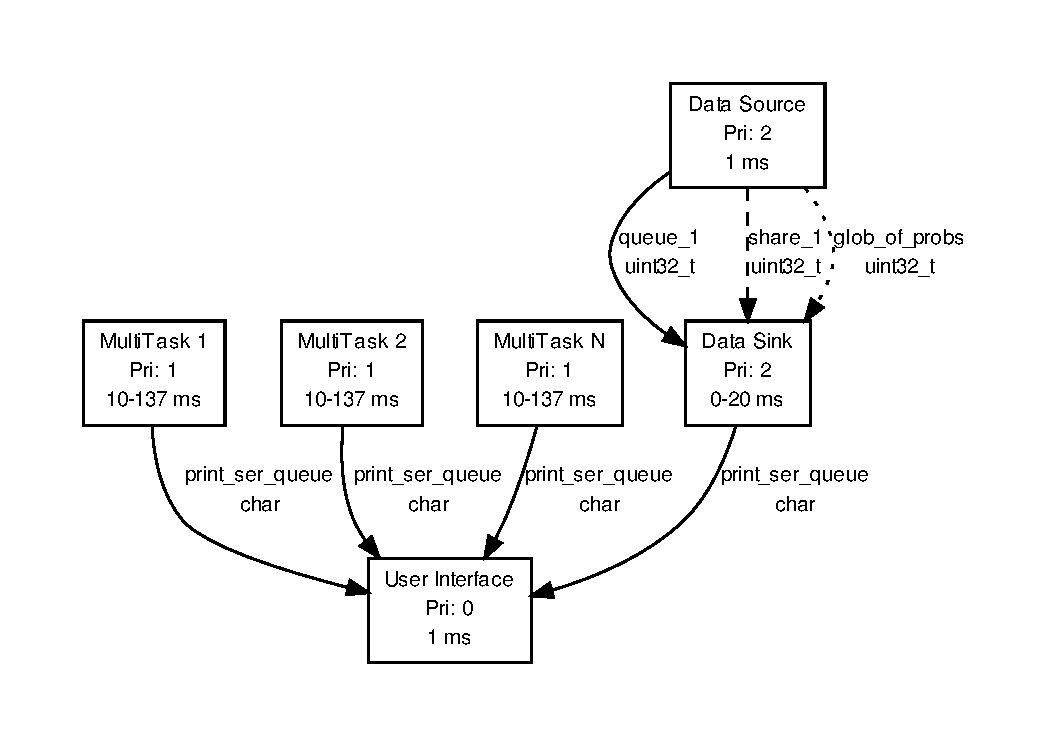
\includegraphics[width=\textwidth,height=\textheight/2,keepaspectratio=true]{dot_inline_dotgraph_1}}
\end{DoxyImageNoCaption}
\end{center}
 There are a couple of unusual features on this task diagram. The number of \char`\"{}multi-\/tasks\char`\"{} can be varied by changing {\ttfamily N\+\_\+\+M\+U\+L\+T\+I\+\_\+\+T\+A\+S\+K\+S} in {\ttfamily \hyperlink{test__main_8cpp_a840291bc02cba5474a4cb46a9b9566fe}{main()}}. These multi-\/tasks are a bunch of tasks, all created from the same class, that are used to put some stress on the R\+T\+O\+S by running lots of tasks at the same time. The multi-\/task's timing includes a delay of random duration; this timing scheme causes tasks to pre-\/empt each other with random timing. The data sink task normally runs very quickly, looking for changed data; if it finds data, it delays by 20 ms to give other tasks some time to run. The data sink therefore takes up a lot of C\+P\+U time, and one can see that the user interface runs slowly because of this.

When this program is running, one can press the \char`\"{}v\char`\"{} key in a terminal window to cause the program to display a task status report. A typical report is shown below. 
\begin{DoxyCode}
Task                            Stack
Name            Pri.    State   Free/Total      Runs
----            ----    -----   ----------      ----
Multi3          1       0       63/120          0        153 runs
Multi2          1       0       63/120          0        161 runs
Multi1          1       0       63/120          0        157 runs
Multi0          1       0       63/120          0        152 runs
UserInt         1       0       66/240          0        4217 runs
Sink            2       0       92/160          0       1136446 runs, errors in queue: 0, shared\_data: 0, 
      global data: 265
Source          2       0       145/220         0        10446 runs
IDLE            0       -       50/100
Heap: 4000/5944, OCR5A=1999
\end{DoxyCode}
 This report shows tasks and their current priorities and states. Also, for the data sink task, it shows a report of how accurately the data from the data source task has been received. One should see that there have been no errors in sending data through the queue or shared data item, but the use of a global variable has caused errors due to task switching while the data was being written or read. 